\section*{Цель работы}

\begin{enumerate}
    \item Получение передаточных характеристик инвертирующего и неинвертирующего усилителей на операционных усилителях;
    \item Исследование их работы.
\end{enumerate}



\section*{Исходные данные}

Все исследования, проводимые в лабораторной работе, выполняются с 
ОУ AD549.

\section*{Построение передаточной характеристики инвертирующего усилителя}

\begin{figure}[H]
    \centering
    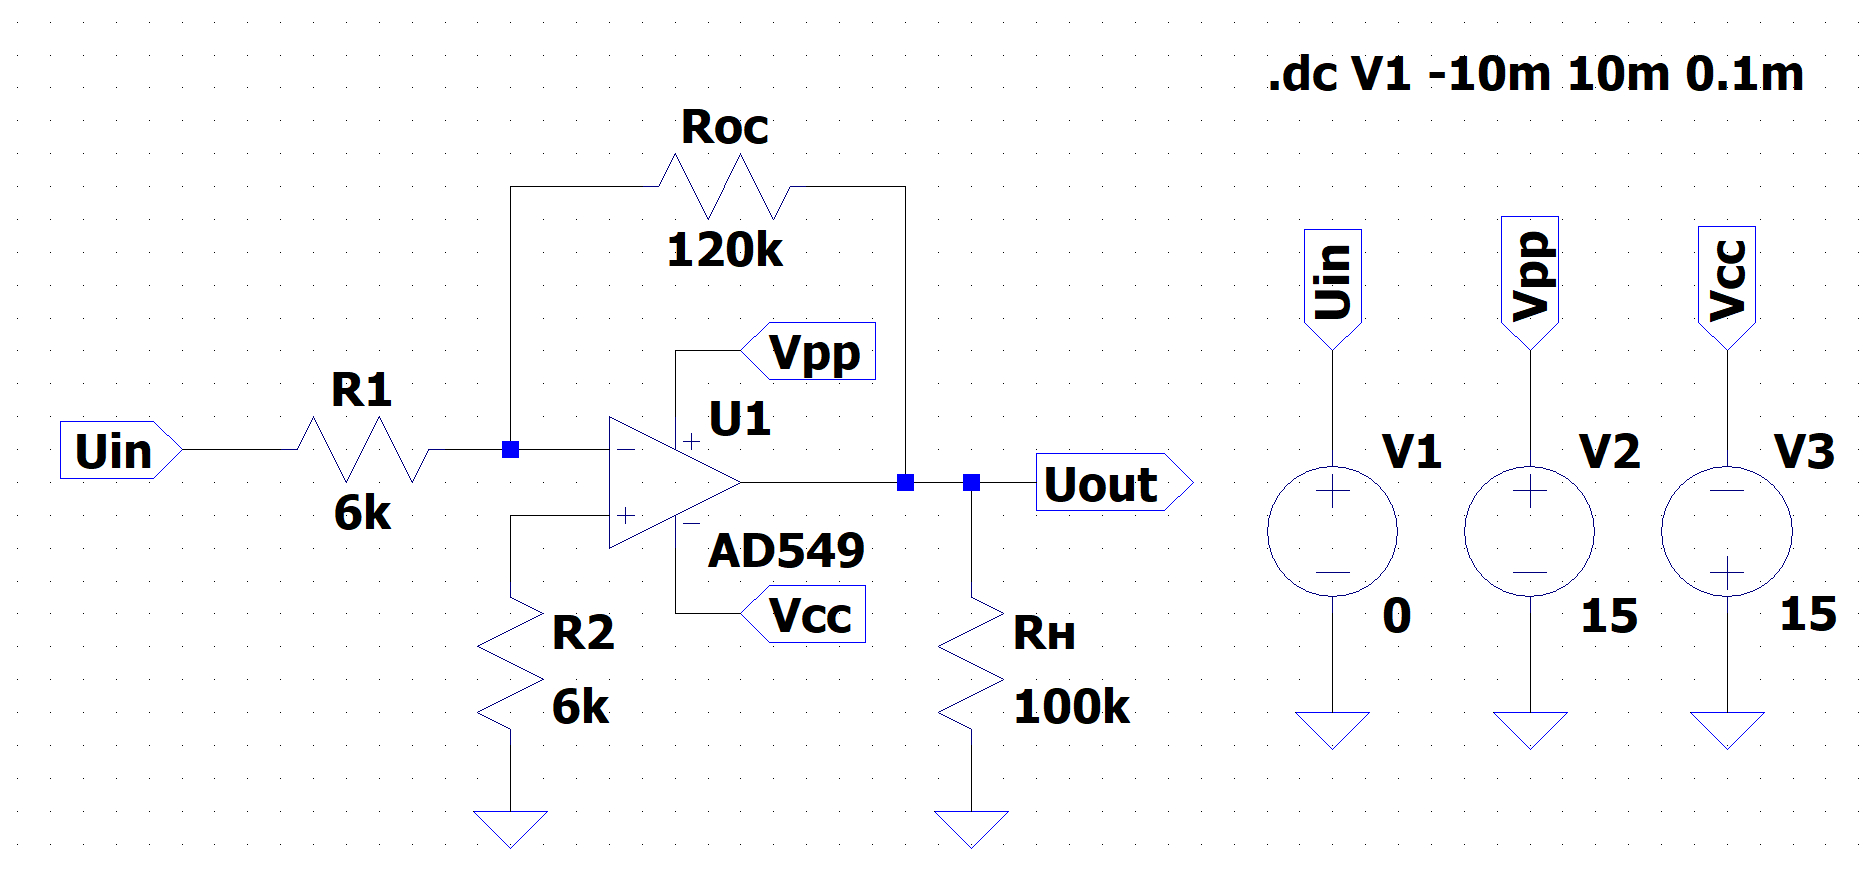
\includegraphics[width=\textwidth]{figs/перед_хар_инв_оу_схема.png}
    \caption{Схема инвертирующего усилителя}
    \label{fig:перед_хар_инв_оу_схема}
\end{figure}

В программе LTspice соберите схему инвертирующего усилителя,
изображенную на рисунке \ref{fig:перед_хар_инв_оу_схема}. Сопротивление обратной
связи $R_{OC}=120k\Omega$ и коэффициент усиления $K=20$ выбраны в соответствии с вариантом.
Затем рассчитаем величину сопротивления резистора $R_1$, используя
формулу
\begin{equation*}
    R_1=\frac{R_{OC}}{K}=6k\Omega. 
\end{equation*}
Сопротивление резистора $R_2$ установим равным сопротивлению резистора $R_1$.

Передаточную характеристику инвертирующего усилителя можно увидеть на рисунке
\ref{fig:перед_хар_инв_оу}. По передаточной характеристике $U_{\text{ОГР+}}=13.40V$, 
$U_{\text{ОГР-}}=-14.15V$, $K=-20.00$.

\begin{figure}[H]
    \centering
    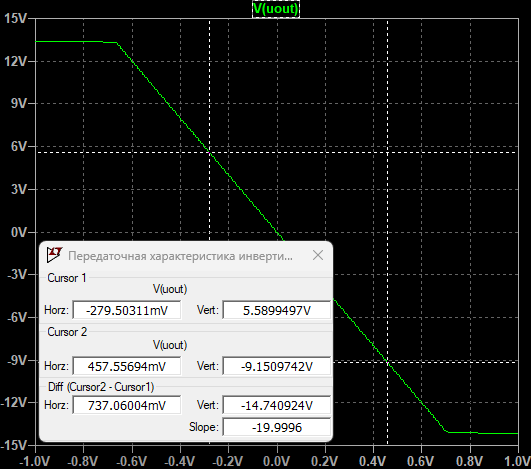
\includegraphics[width=\textwidth]{figs/перед_хар_инв_оу.png}
    \caption{Передаточная характеристика инвертирующего усилителя}
    \label{fig:перед_хар_инв_оу}
\end{figure}

\section*{Исследование работы инвертирующего усилителя}

В схеме (см. рис. \ref{fig:перед_хар_инв_оу_схема}) на вход усилителя подадим 
синусоидальный сигнал частотой 50 Гц. Амплитуду установим $0.5$ В, чтобы амплитуда
сигнала на выходе лежала в пределах напряжения ограничения. Осциллограммы входного
и выходного напряжения можно увидеть на рисунке \ref{fig:иссл_раб_инв_усл}.

Как можно видеть выходной сигнал и входной находятся в противофазе. 
Амплитуда выходного сигнала составляет $9.99$ В, найдем
коэффициент усиления:
\begin{equation*}
    K=\frac{9.99}{0.5}=19.98\ .
\end{equation*}
Этот коэффициент отличается от модуля ранее рассчитанного коэффициента на 0.1\%.
Сам же этот коэффициент отличается от заданого в таблице только знаком.

\begin{figure}[H]
    \centering
    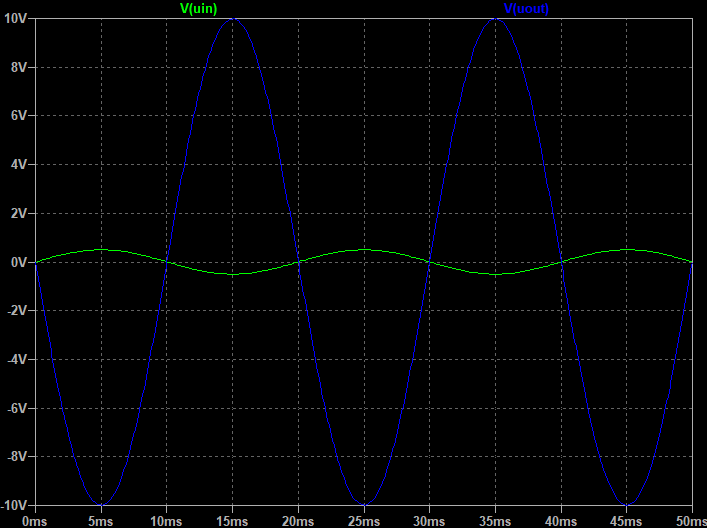
\includegraphics[width=\textwidth]{figs/иссл_раб_инв_усл.png}
    \caption{Осциллограммы входного
    и выходного напряжения при грамоническом входе инвертирующего усилителя}
    \label{fig:иссл_раб_инв_усл}
\end{figure}


\section*{Построение передаточной характеристики неинвертирующего усилителя}

В программе LTspice соберите схему неинвертирующего усилителя,
изображенную на рисунке \ref{fig:перед_хар_неинв_оу_схема}. Рассчитаем величину сопротивления резистора $R_1$, 
используя формулу
\begin{equation*}
    R_1=\frac{R_{OC}}{K-1}\approx 6315.79\ \Omega.
\end{equation*}
Сопротивление резистора $R_2$ установим равным сопротивлению резистора $R_1$.

Передаточную характеристику неинвертирующего усилителя можно увидеть на рисунке
\ref{fig:перед_хар_неинв_оу}. По передаточной характеристике $U_{\text{ОГР+}}=13.41V$, 
$U_{\text{ОГР-}}=-14.16V$, $K=20.00$.

\begin{figure}[H]
    \centering
    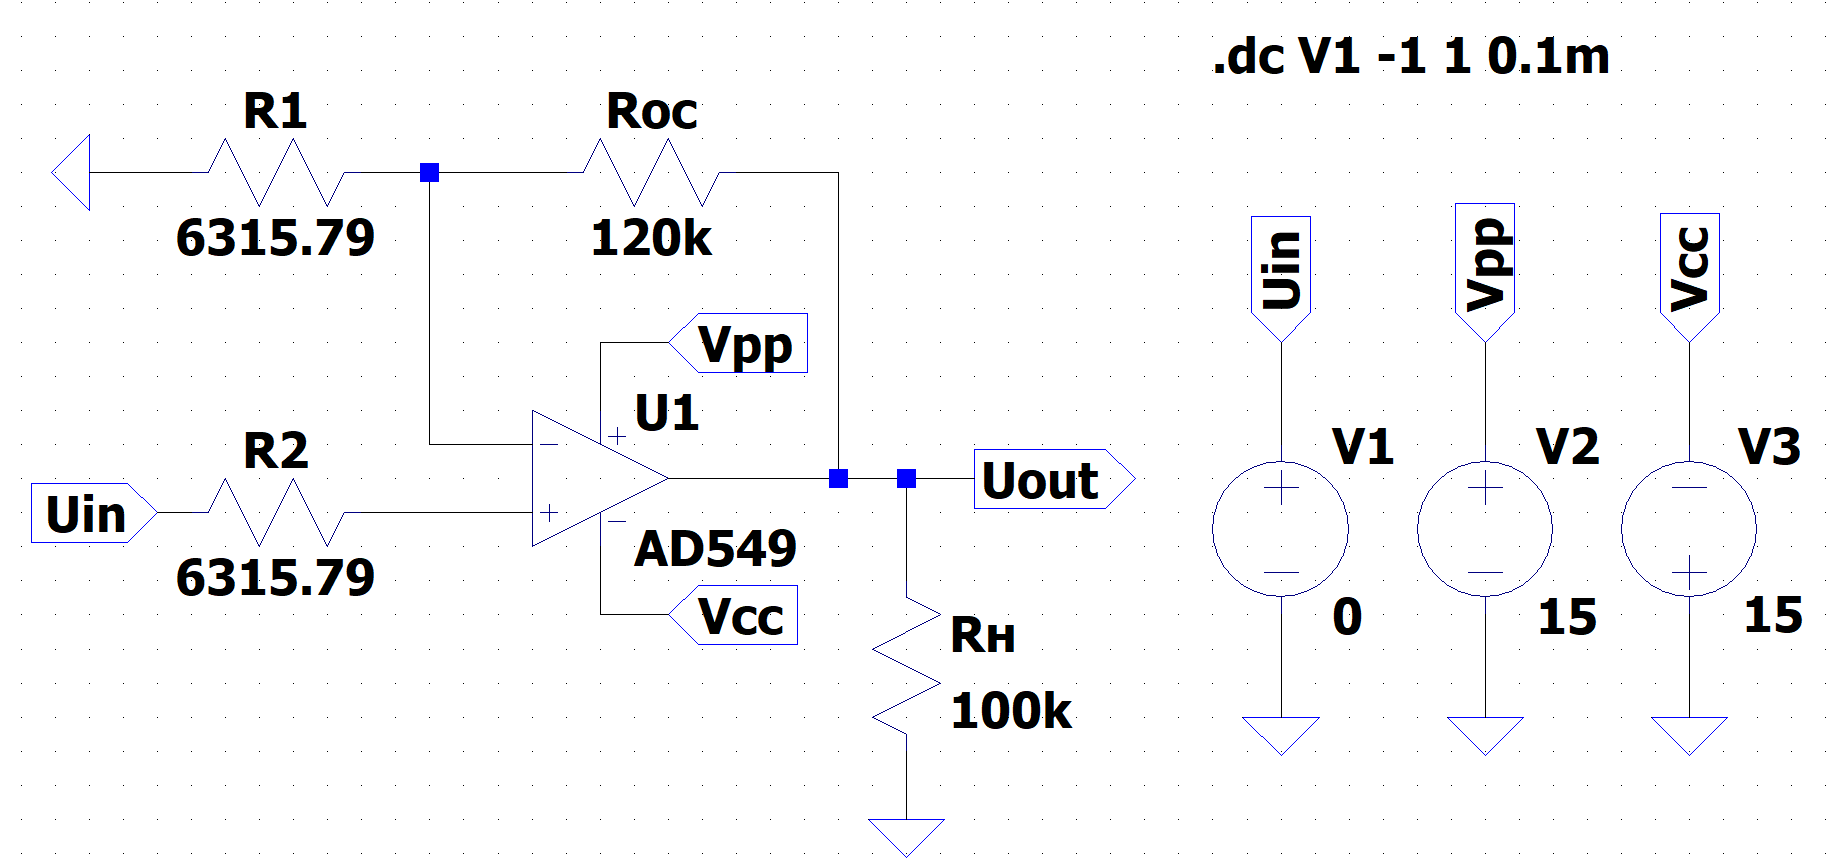
\includegraphics[width=\textwidth]{figs/перед_хар_неинв_оу_схема.png}
    \caption{Схема неинвертирующего усилителя}
    \label{fig:перед_хар_неинв_оу_схема}
\end{figure}

\begin{figure}[H]
    \centering
    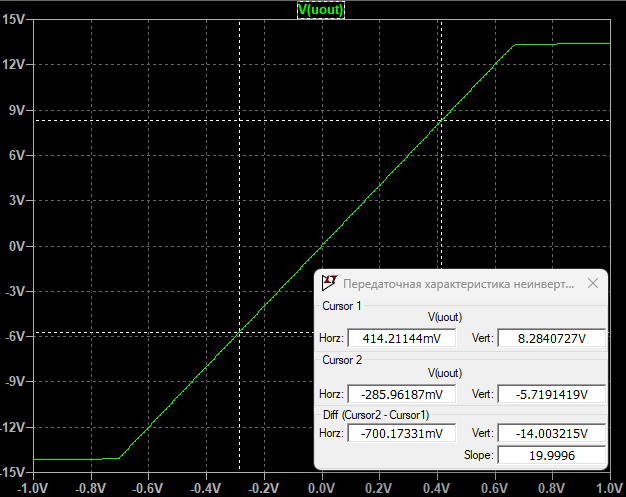
\includegraphics[width=\textwidth]{figs/перед_хар_неинв_оу.png}
    \caption{Передаточная характеристика неинвертирующего усилителя}
    \label{fig:перед_хар_неинв_оу}
\end{figure}


\section*{Исследование работы неинвертирующего усилителя}

В схеме (см. рис. \ref{fig:перед_хар_неинв_оу_схема}) на вход усилителя подадим 
синусоидальный сигнал частотой 50 Гц. Амплитуду установим $0.5$ В, чтобы амплитуда
сигнала на выходе лежала в пределах напряжения ограничения. Осциллограммы входного
и выходного напряжения можно увидеть на рисунке \ref{fig:иссл_раб_неинв_усл}.

Как можно видеть фаза выходного сигнала несмещена относительно фазы входного сигнала. 
Амплитуда выходного сигнала составляет $9.99$ В, найдем
коэффициент усиления:
\begin{equation*}
    K=\frac{9.99}{0.5}=19.98\ .
\end{equation*}
Этот коэффициент отличается от ранее рассчитанного коэффициента на 0.1\%.
Сам же этот коэффициент не отличается от заданого в таблице.

\begin{figure}[H]
    \centering
    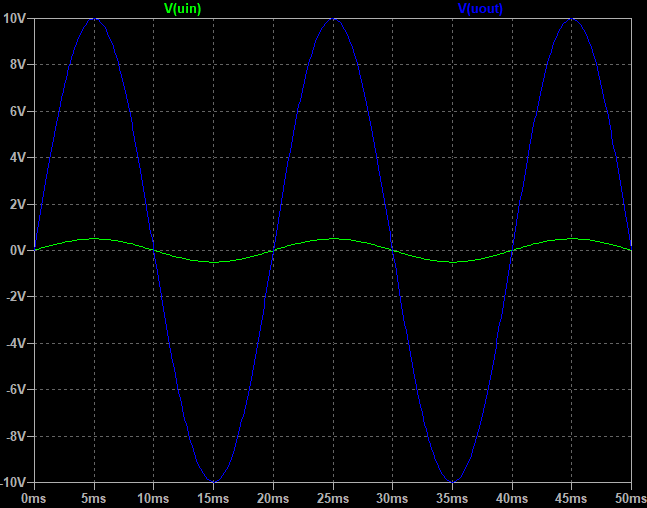
\includegraphics[width=\textwidth]{figs/иссл_раб_неинв_усл.png}
    \caption{Осциллограммы входного
    и выходного напряжения при грамоническом входе неинвертирующего усилителя}
    \label{fig:иссл_раб_неинв_усл}
\end{figure}


\section*{Заключение}

В ходе работы были исследованы схемы инвертирующего и неинвертирующего усилителей
на операционном усилителе AD549. Были получены их передаточные характеристики.

